\documentclass[9pt]{article}

\usepackage{amssymb}
\usepackage{amsmath}
\usepackage{amsfonts}
\usepackage{comment}
\usepackage{fancyhdr}
\usepackage{mathrsfs}
\usepackage{enumitem}
\usepackage{graphicx}

\usepackage{tikz}

\voffset = -50pt
%\textheight = 700pt
\addtolength{\textwidth}{60pt}
\addtolength{\evensidemargin}{-30pt}
\addtolength{\oddsidemargin}{-30pt}
%\setlength{\headheight}{44pt}

\newcommand{\qed}{\hfill \ensuremath{\Box}}


\newcommand*\circled[1]{\tikz[baseline=(char.base)]{
            \node[shape=circle,draw,inner sep=2pt] (char) {#1};}}

\newcommand{\Z}{\mathbb{Z}}
\newcommand{\I}{\mathbb{I}}
\newcommand{\M}{\mathbb{M}}
\newcommand{\R}{\mathbb{R}}
\newcommand{\C}{\mathbb{C}}
%\setcounter{section}{-1}

\begin{document}
\topskip0pt
\vspace*{\fill}
\begin{center}
{\Huge \begin{tabular}{@{}ll@{}}
   Class: & CECS 201, Section 7 \\ \\ \\
   Lab: & 5 \\ \\ \\
   Title: & Logic Simplification \\ \\ \\
   Student Name: & Barry Joseph Okonoboh \\ \\ \\
   Due Date: & 07:00:00 P.M., 16, March 2015 \\ \\ \\
   Instructor: & Dan Cregg
\end{tabular}}
\end{center}
\vspace*{\fill}
\newpage
\begin{enumerate}
%%%%%%%%%%%%%%%%%%%%%%%%%%%%%%%%%%%%%%%%01%%%%%%%%%%%%%%%%%%%%%%%%%%%%%%%%%%%%%%
   \item[\textbf{Introduction.}]  This lab involves simplifying complex
   circuits using Boolean Algebra and Karnaugh Maps.
   \item[\textbf{Project Description.}]  We use Boolean Algebra and Karnaugh
   maps to simplify an equation. Then we draw two circuits on a schematic, one
   which represents the unsimplified equation, and the order that represents the
   simplified equation. Upon observing the program on the Digilent board, one should
   observe that  for the same input, both circuits return the same output.
  	\item[\textbf{Schematic Part 1.}] \text{ }
   
             \begin{center}
                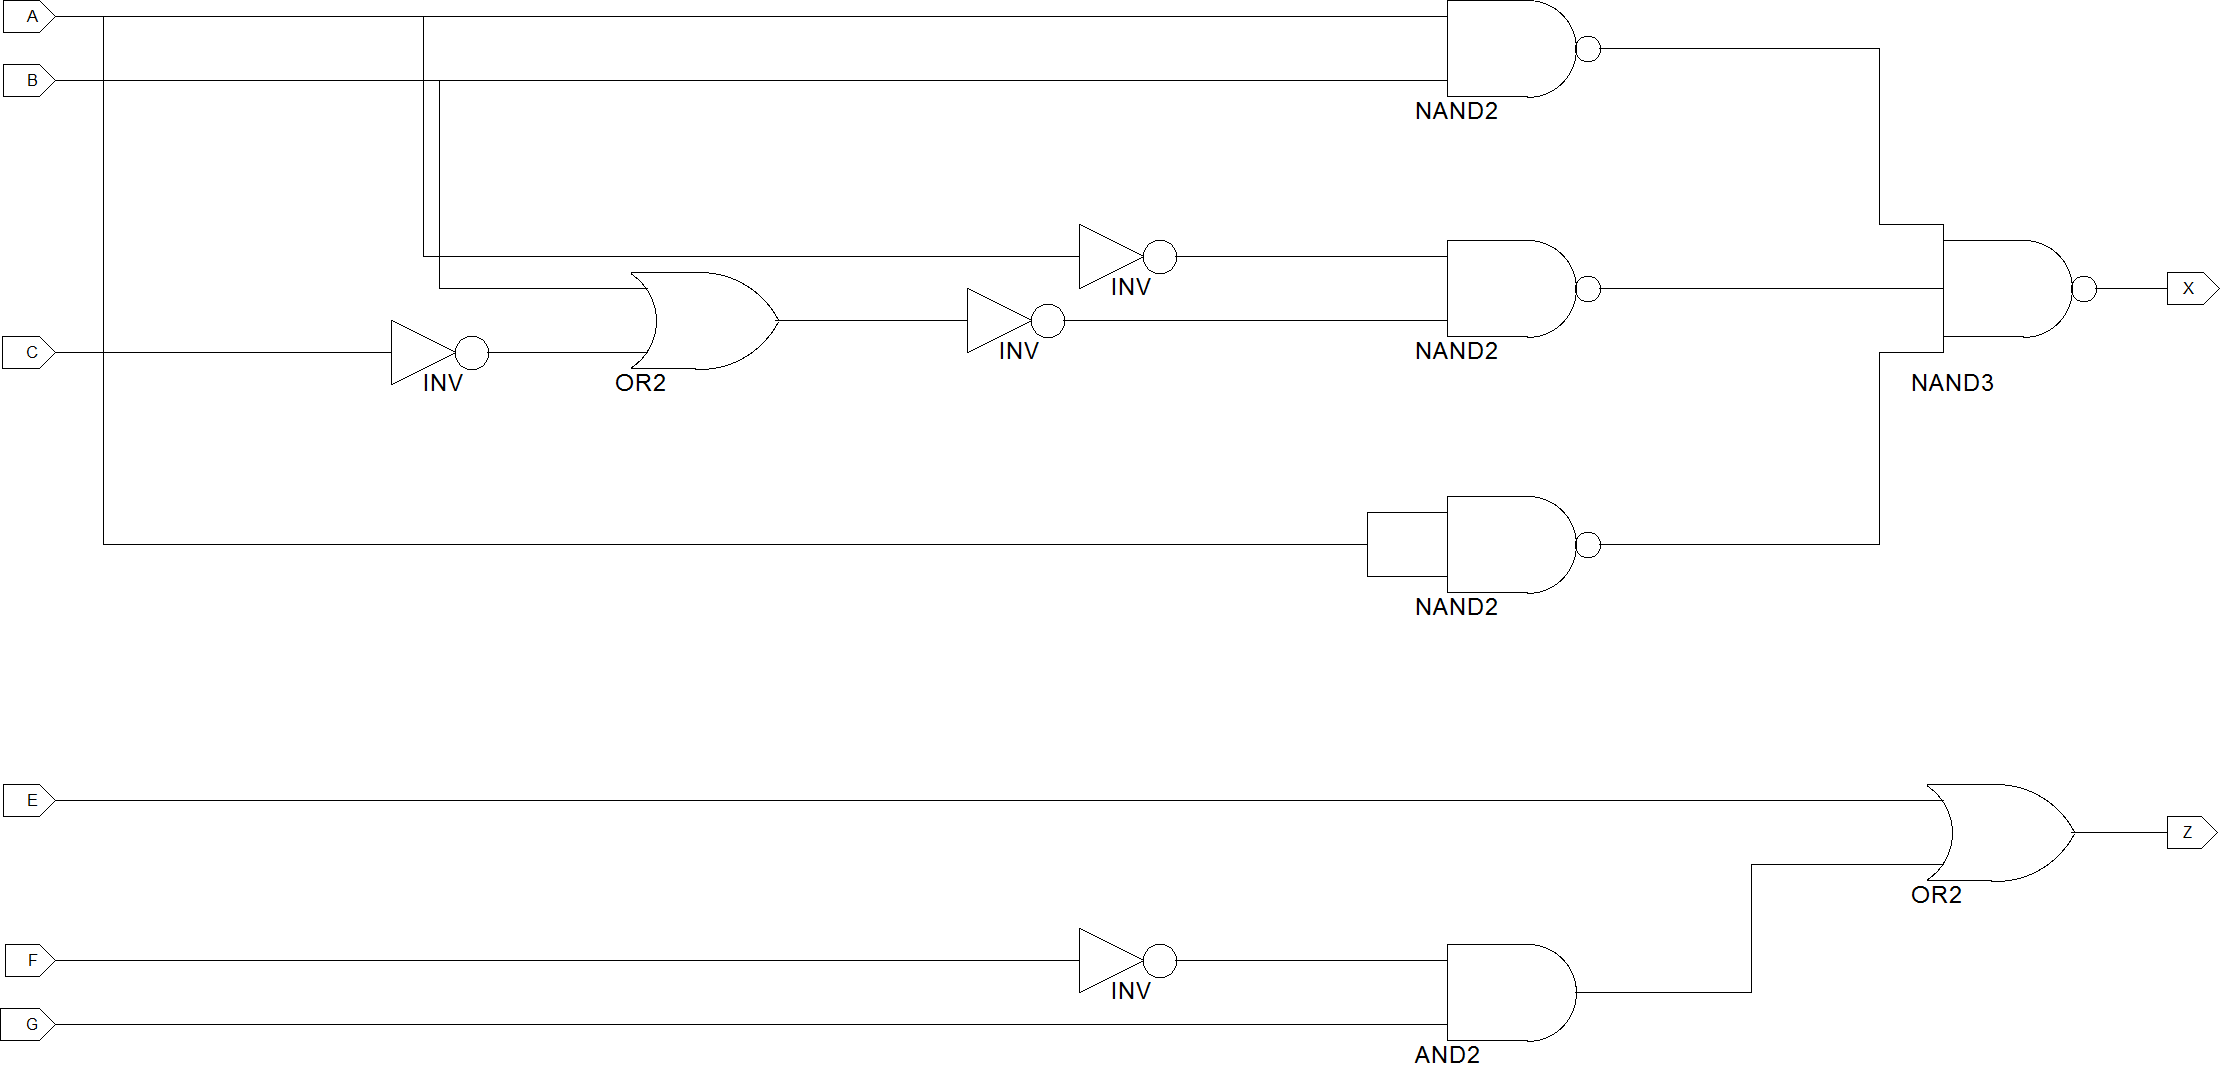
\includegraphics[width=\textwidth]{schematic.png}
             \end{center}
   
  	\item[\textbf{Schematic Part 2.}] \text{ }
   
             \begin{center}
                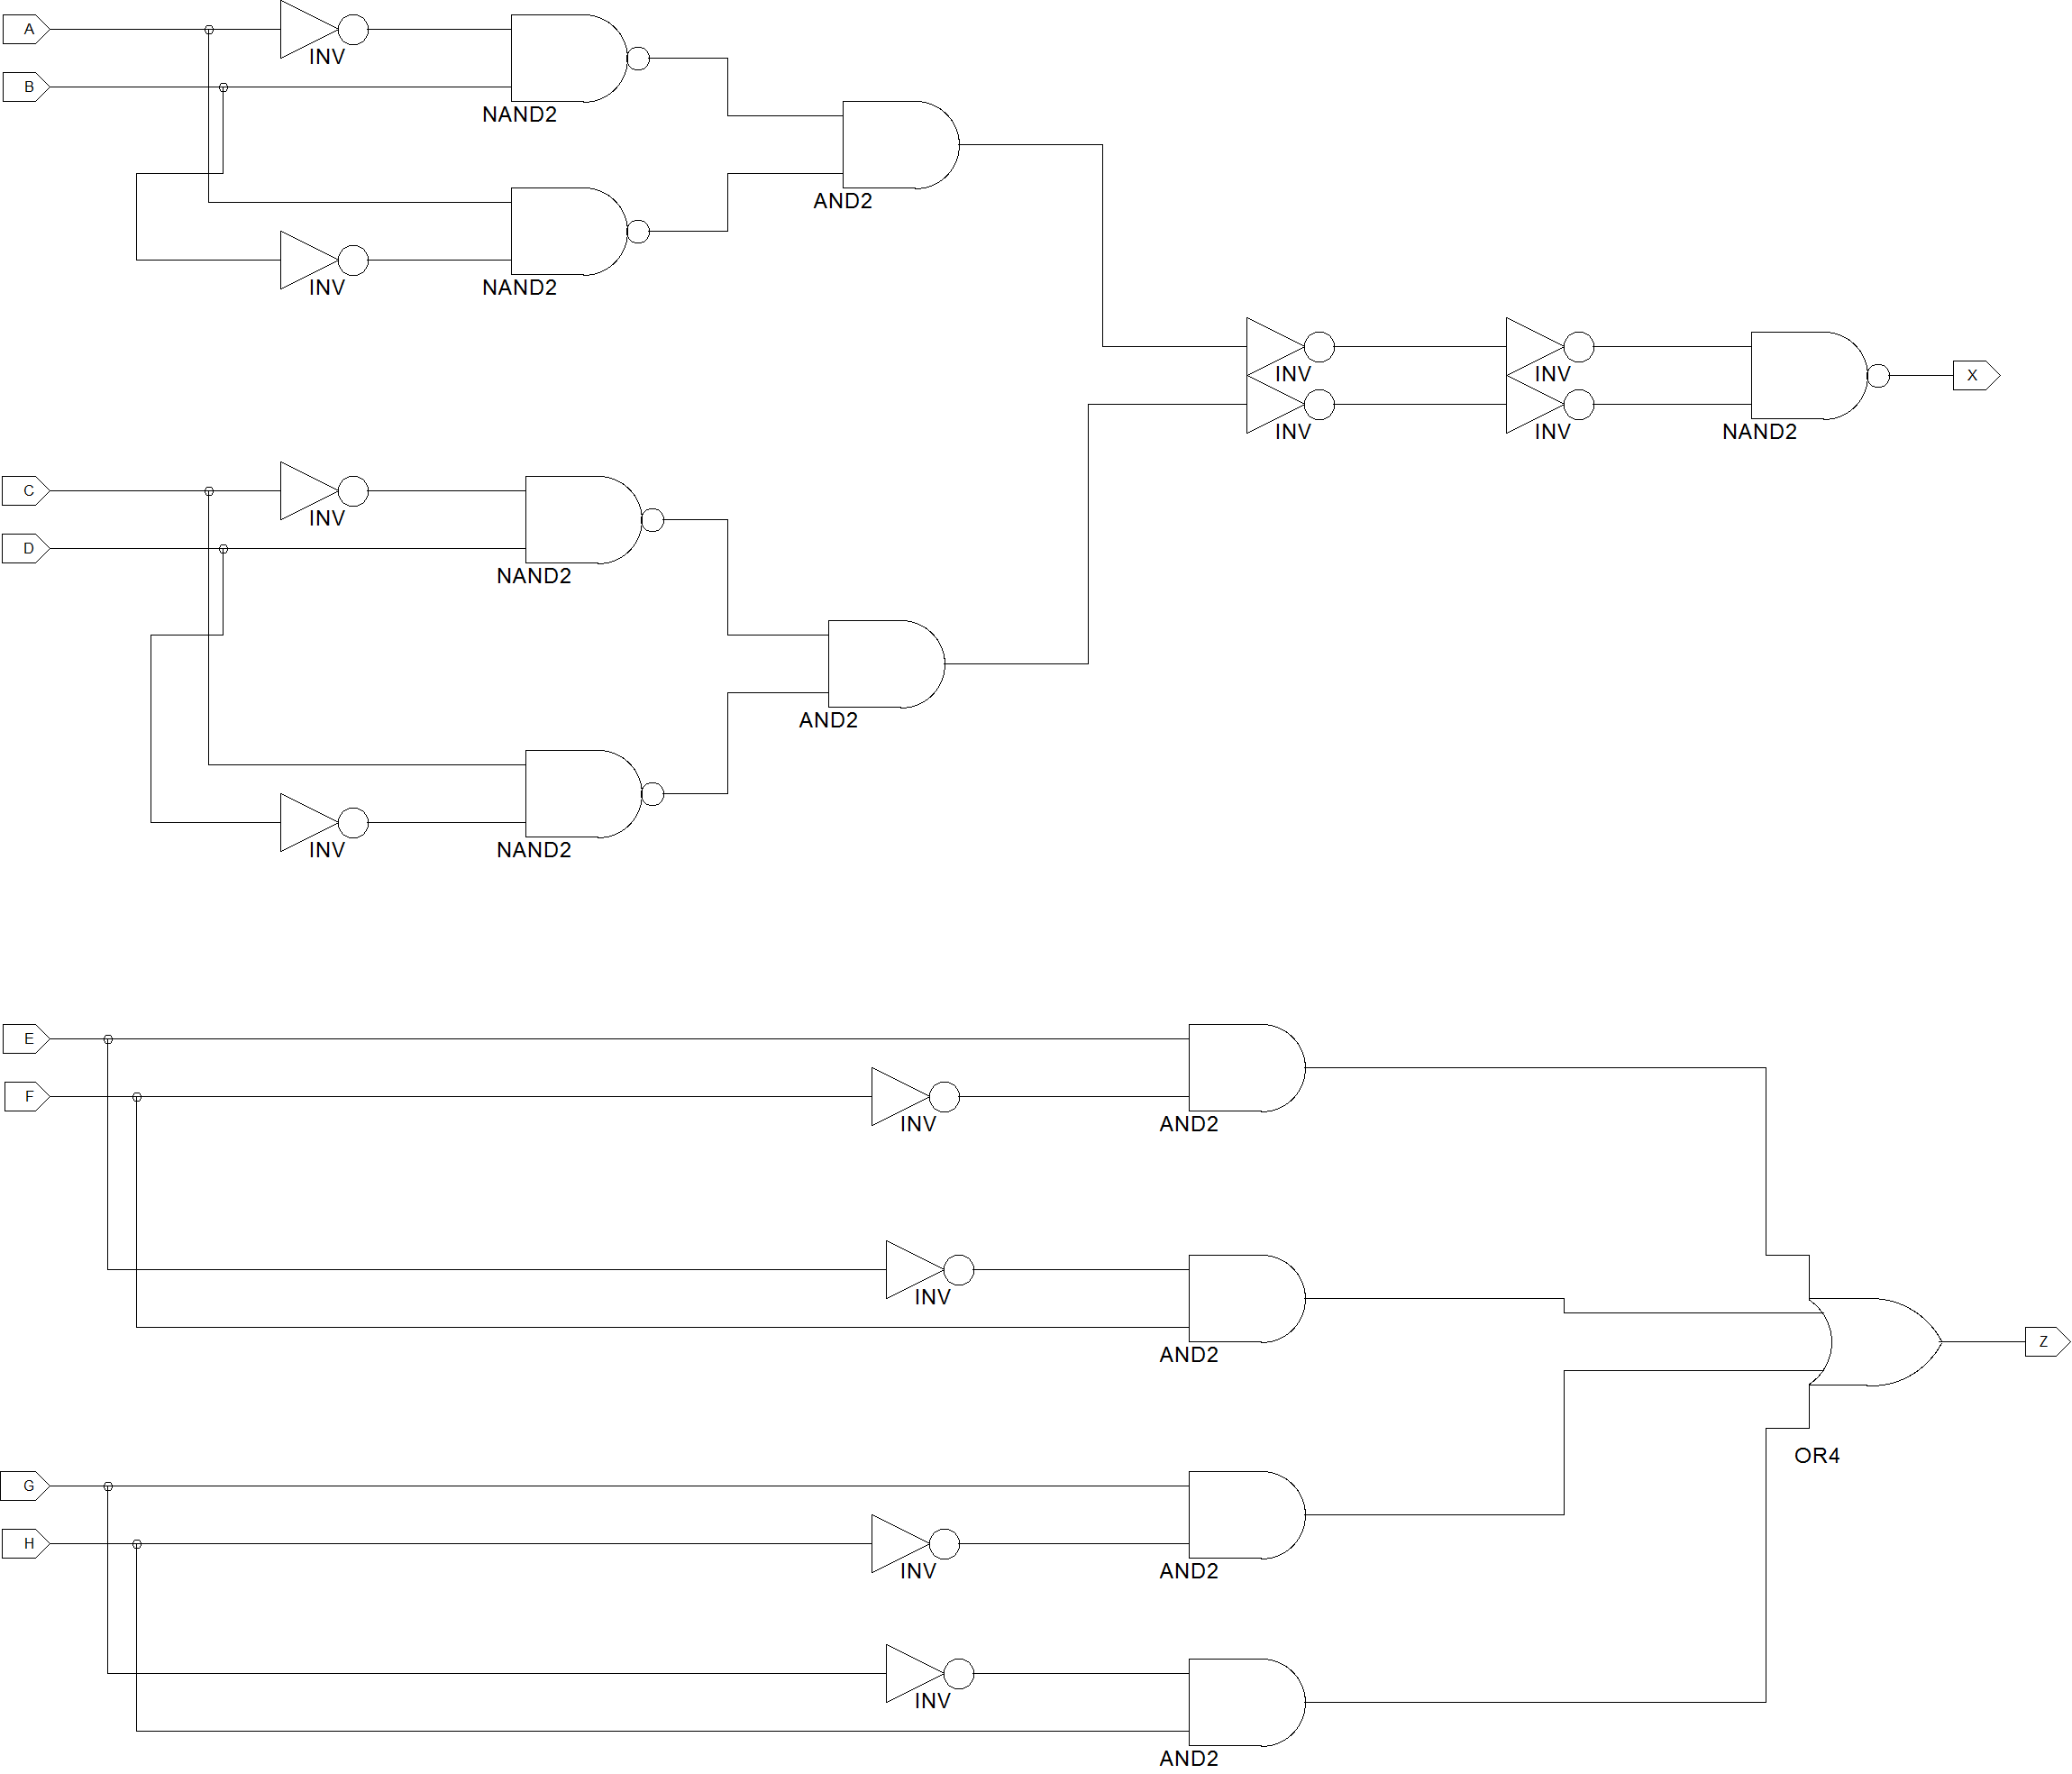
\includegraphics[width=\textwidth]{schematicp2.png}
             \end{center}
   \item[Part 1.] We wish to reduce $X = ((AB)'(A'(B + C')')'(A)')'$ to sum of
             products. Thus
             \begin{align*}
               X &= ((AB)'(A'(B + C')')'(A)')' \\
                 &= (AB)'' + (A'(B + C')')'' + (A)'' \\
                 &= AB + A'(B + C')' + A \\
                 &= AB + A'(B'C'') + A \\
                 &= AB + A'B'C + A\\
                 &= AB + A + A'B'C \\
                 &= A(B + 1) + A'B'C \\
                 &= A + A'B'C.
             \end{align*}             
             
            We have the following truth table of the equation $X = A + A'B'C$:
            \begin{center}
            \begin{tabular}{@{}|c|c|c|c|@{}}
            \hline
            $A$ & $B$ & $C$ & $X$ \\ \hline
            0 & 0 & 0 & 0 \\ \hline
            0 & 0 & 1 & 1 \\ \hline
            0 & 1 & 0 & 0 \\ \hline
            0 & 1 & 1 & 0 \\ \hline
            1 & 0 & 0 & 1 \\ \hline
            1 & 0 & 1 & 1 \\ \hline
            1 & 1 & 0 & 1 \\ \hline
            1 & 1 & 1 & 1 \\ \hline
\end{tabular}
\end{center}

            Using Karnaugh map, we have that
            \begin{center}
            \begin{tabular}{@{}|c|c|c|c|c|@{}}
            \hline
            & \textbf{00} & \textbf{01} & \textbf{11} & \textbf{10} \\ \hline
            \textbf{0} & 0 & 1 & 0 & 0 \\ \hline
            \textbf{1} & 1 & 1 & 1 & 1 \\
            \hline
\end{tabular}
            \end{center}
            
            so that $X = A + B'C$.
   \item[Part 2.] We now wish to reduce the equation
                 $X = (((A'B)'(B'A)')'' ((C'D)'(CD')')'')'$ to sum of
             products. Thus
             \begin{align*}
               X &= (((A'B)'(B'A)')'' ((C'D)'(CD')')'')' \\
                 &= (((A'B)'(B'A)') ((C'D)'(CD')'))' \\
                 &= (((A'' + B')(B'' + A')) ((C'' + D')(C' + D'')))' \\
                 &= (((A + B')(B + A')) ((C + D')(C' + D)))' \\
                 &= ((A + B')(B + A'))' + ((C + D')(C' + D))' \\
                 &= (A + B')' + (B + A')' + (C + D')' + (C' + D)' \\
                 &= A'B'' + B'A'' + C'D'' + C''D' \\
                 &= A'B + B'A + C'D + CD'.
             \end{align*}             
             
            We have the following truth table of the equation
            $X = A'B + B'A + C'D + CD'$:
            \begin{center}
            \begin{tabular}{@{}|c|c|c|c|c|c|c|@{}}
            \hline
            $A$ & $B$ & $C$ & $D$ & $A'B + B'A$ & $C'D + CD'$ & X\\ \hline
            0 & 0 & 0 & 0 & 0 & 0 & 0 \\ \hline
            0 & 0 & 0 & 1 & 0 & 1 & 1 \\ \hline
            0 & 0 & 1 & 0 & 0 & 1 & 1 \\ \hline
            0 & 0 & 1 & 1 & 0 & 0 & 0 \\ \hline
            0 & 1 & 0 & 0 & 1 & 0 & 1 \\ \hline
            0 & 1 & 0 & 1 & 1 & 1 & 1 \\ \hline
            0 & 1 & 1 & 0 & 1 & 1 & 1 \\ \hline
            0 & 1 & 1 & 1 & 1 & 0 & 1 \\ \hline
            1 & 0 & 0 & 0 & 1 & 0 & 1 \\ \hline
            1 & 0 & 0 & 1 & 1 & 1 & 1 \\ \hline
            1 & 0 & 1 & 0 & 1 & 1 & 1 \\ \hline
            1 & 0 & 1 & 1 & 1 & 0 & 1 \\ \hline
            1 & 1 & 0 & 0 & 0 & 0 & 0 \\ \hline
            1 & 1 & 0 & 1 & 0 & 1 & 1 \\ \hline
            1 & 1 & 1 & 0 & 0 & 1 & 1 \\ \hline
            1 & 1 & 1 & 1 & 0 & 0 & 0 \\ \hline
\end{tabular}
\end{center}

            Using Karnaugh map, we have that
            \begin{center}
            \begin{tabular}{@{}|c|c|c|c|c|@{}}
            \hline
            & \textbf{00} & \textbf{01} & \textbf{11} & \textbf{10} \\ \hline
            \textbf{00} & 0 & 1 & 0 & 1 \\ \hline
            \textbf{01} & 1 & 1 & 1 & 1 \\ \hline
            \textbf{11} & 0 & 1 & 0 & 1 \\ \hline
            \textbf{10} & 1 & 1 & 1 & 1 \\
            \hline
\end{tabular}
            \end{center}
            
            so that $X = A'B + AB' + C'D + CD'$.
\end{enumerate}
\end{document}